\chapter{Asterisk, an open source PBX}
\section{Overview}
Created in 1999, Asterisk is designed to be an open-source telephony server. Multi-platform, it can be used in lot of various application. It can also easily manage both physical phone devices and phones software. More globally, a PBX is able to create automated vocal services, internal company phone service, voice mails... And it is just some examples of a PBX usage.

\section{Why Asterisk?}
For this project, we tried to look for an efficient telephony server. A server with a lot of documentation and a great community support would be ideal. Moreover, this server should be really flexible because the configuration will be often generated, and then reloaded.
Because lot of these PBX are managed by a web GUI interface, we discovered \textit{Asterisk}. It seemed to be the ideal server we needed. It have an excellent community support, a great documentation and able to reload its configuration fastly without interrupting current communications.

\section{Server compilation}
Because \textit{Asterisk} is provided as open source server, we had to download the server sources and then compile them with the following commands:
\begin{lstlisting}[language=bash,caption={bash}]
\end{lstlisting}

One of the most important command in the above list was \textit{make menuselect}: this command allows to enable and disable unwanted modules. It is there we can enable for example the MP3 support.

\section{Server organization}

\subsection{Contexts}
On Asterisk, all phone activities are based on contexts. It means when a phone is registered in a context, it can't reach phones which are located in different context. The contexts will be mainly useful for the company switchboard. Indeed, all switchboard will have their own context called like "\textbf{SWITCHBOARD\_USER\_(CODE)}" where (CODE) is replaced by the switchboard access code, defined at the creation of the switchboard on the website.


\textit{ScotIP} purposes two kinds of lines: the dedicated line and the shared lines.
Shared lines will share the same starting context. It is a vocal service where all incoming calls will be redirected. This vocal service will ask the caller to enter the switchboard access code, and if it exists, then the caller will be redirected on the switchboard context.


This is possible thanks to variables, conditions and functions provided in Asterisk. When the caller will press his phone keys, the number will be stored in a temporary variable. Then, thanks to the function \textbf{DIALPLAN\_EXISTS(name)} the caller can be redirected on the right context. Otherwise, the call will be hang up. 

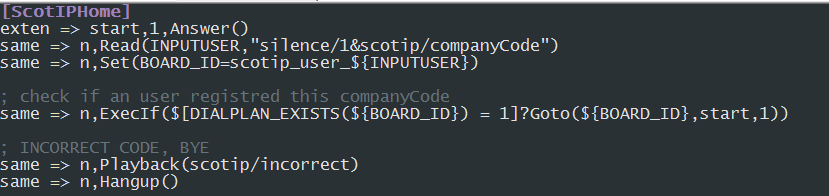
\includegraphics[width=1\textwidth]{img/context_scotiphome.png}


\subsection{Files}


\section{SIP}

\subsection{SIP peers}
Parler ici des connexions OVH, IPPI
\subsection{Extensions}
Create operators, phones...


\section{Dialplan}

Queue
Operator
Playback

Phone keys
User input


\section{MOH}
 